
\documentclass{beamer}


\mode<presentation> 
	{
	%\usetheme{Berlin}
	%\usetheme{Copenhagen}
	%\usetheme{Luebeck}
	\usetheme{Madrid}
	\setbeamertemplate{navigation symbols}{} 
	\setbeamertemplate{itemize item}[square]
	\setbeamertemplate{itemize subitem}[square]
	\setbeamertemplate{caption}{\raggedright\insertcaption\par}
	\setbeamerfont{footnote}{size=\tiny}

	%\makeatletter
	\setbeamercolor{footline}{fg=white, bg=darkblue}
	\setbeamertemplate{footline}
	{
	  \leavevmode%
	  \hbox{%
	  \begin{beamercolorbox}[wd=.25\paperwidth,ht=2.25ex,dp=1ex,center]{footline}%
	    \usebeamerfont{author in head/foot}\insertauthor\hspace*{1em}
	  \end{beamercolorbox}%
	  \begin{beamercolorbox}[wd=.50\paperwidth,ht=2.25ex,dp=1ex,center]{footline}%
	    \usebeamerfont{title in head/foot}\insertshorttitle
	  \end{beamercolorbox}%
	  \begin{beamercolorbox}[wd=.25\paperwidth,ht=2.25ex,dp=1ex,right]{footline}%
	    \usebeamerfont{date in head/foot}\insertshortdate{}\hspace*{2em}
	  \end{beamercolorbox}}%
	  \vskip0pt%
	}
	%\makeatother

	}

\usepackage{graphicx} 
\usepackage{booktabs}
\usepackage{textcomp} 

\usepackage{tcolorbox}
\usepackage{amsmath,amssymb}

\newcommand\blfootnote[1]{%
  \begingroup
  \renewcommand\thefootnote{}\footnote{#1}%
  \addtocounter{footnote}{-1}%
  \endgroup
}

\definecolor{darkblue}{RGB}{32, 76, 129}
\setbeamercolor{frametitle}{bg=darkblue, fg=white}




%----------------------------------------------------------------------------------------
%	TITLE PAGE
%----------------------------------------------------------------------------------------

\title[Activity Intensity in Social Network Communities]{Activity Intensity in Social Network Communities:  \\ a case study} 

\author{Matteo Garbellini} 
\institute[(UniMi)] 
{
Universit\`a degli Studi di Milano \\ 
\medskip
}
\titlegraphic{
\includegraphics[width=2cm]{unimi}}
\date{23 Luglio 2019} 

\begin{document}

{
%\usebackgroundtemplate{\includegraphics[width=\paperwidth]{fig7_70.jpg}}%
\begin{frame}
\titlepage
\end{frame}
}

%----------------------------------------------------------------------------------------
%	PRESENTATION SLIDES
%----------------------------------------------------------------------------------------

%\begin{frame}
%\frametitle{Overview}
%\tableofcontents
%\end{frame}

\section{Introduction}
\subsection{Context}
\subsection{Question}
\subsection{Dataset}
\section{Methods}
\section{Results}
\section{Conclusions}
%------------------------------------------------

\begin{frame}
\frametitle{Introduction}
{
\vspace{-0.3cm}
\centering
\begin{tcolorbox}[width=6cm, colframe=white, colback=white, halign=center]
\Large Analysis of the Activity in a Social Network
\end{tcolorbox}
}
	
\vspace{0.5cm}

\begin{columns}
	\begin{column}[T]{0.4\textwidth}
	\textbf{The Anatomy of a Scientific Rumor}, M. De Domenico et al. \\ \textit{Nature, Scientific Reports, 2013}
	\begin{itemize}
		\item Study of user activity at a global level
	\end{itemize}
	\end{column}

	\begin{column}[T]{0.55\textwidth}
	\textbf{Principal Pattern on Graphs: discovering coherent structures in dataset}, K. Benzi et al. \textit{IEEE Transactions on Signal and Information Processing over Networks, 2016}
	\begin{itemize}
		\item Study of activity pattern and communities dynamics
	\end{itemize}
	\end{column}
\end{columns}
\vspace{0.5cm}
{
\centering
\begin{tcolorbox}[width=8.5cm, colframe=blue, colback=white, halign=center]
\Large Study of the activity at a local level
\end{tcolorbox}
} 
\end{frame}
%------------------------------------------------

\begin{frame}
\frametitle{Goal of the study}
{
\centering
\begin{tcolorbox}[width=10cm, colframe=black, colback=white, halign=center]
\Large Analyze the difference in \textbf{activity intensity} between \textbf{small} and \textbf{large} communities
\end{tcolorbox}
} 

\begin{itemize}
	\setlength{\itemindent}{1cm}
	\vspace{0.5cm} \Large 
	\item \Large Type of interaction between communities
	\vspace{0.5cm} 
	\item \Large Type of interaction between users
\end{itemize}

\end{frame}

%------------------------------------------------

\begin{frame}
\frametitle{Context}

\begin{columns}
	\begin{column}{0.6\textwidth}
	\begin{itemize}
		\item \textbf{Social Network}: Twitter \\following/followers relationships
		\vspace{0.6cm}
		\item \textbf{Communities} of Users
		\vspace{0.6cm}
		\item Study of community \textbf{activity} during \textbf{extraordinary event} \\ \vspace{0.3cm} \hspace{1cm} \textbf{\textrightarrow}   Discovery of the Higgs Boson 

	\end{itemize}
	\end{column}
	\begin{column}{0.4\textwidth}
		\begin{figure}
		
\includegraphics[width=0.6\linewidth]{figures/twitter_logo}
		\end{figure}
	\end{column}
\end{columns}
\end{frame}

%------------------------------------------------

\begin{frame}
\frametitle{Higgs Dataset}
Twitter activity during the announcement of the discovery of the Higgs Boson on July 12th 2012

\begin{columns}
\begin{column}{0.6\textwidth}
\begin{itemize}
	\item \textbf{Time interval} \\ From July 11th 00:00 to July 12th 23:59
	\item \textbf{Directed following/followers network} \\ 450000 users and 14 million edges \\\vspace{0.3cm}\hspace{0.5cm}userID $->$ userID \vspace{0.3cm}
	\item \textbf{Timestamped interactions} \\ 500000 events \\ \vspace{0.2cm}\hspace{0.5cm}userID   userID   timestamp   Retweet\\
	\hspace{0.5cm}userID userID timestamp Mention
\end{itemize}
\end{column}
\begin{column}{0.3\textwidth}
	\begin{figure}
	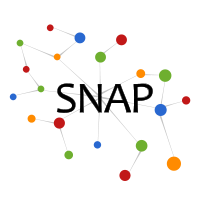
\includegraphics[width=0.9\linewidth]{figures/snap}
	\end{figure}
\end{column}
\end{columns}
\blfootnote{\small Source: SNAP Datasets, Stanford Large Network Dataset Collection}
\end{frame}

%------------------------------------------------

\begin{frame}
\frametitle{What defines a community?}
\begin{columns}
	\begin{column}{0.47\textwidth}
		\begin{itemize}
			\item Very dense connections between users within community
			\vspace{1cm}
			\item Very sparse connection coming in and going out community
		\end{itemize}
	\end{column}
	\begin{column}{0.5\textwidth}
		\begin{figure}
		\centering
			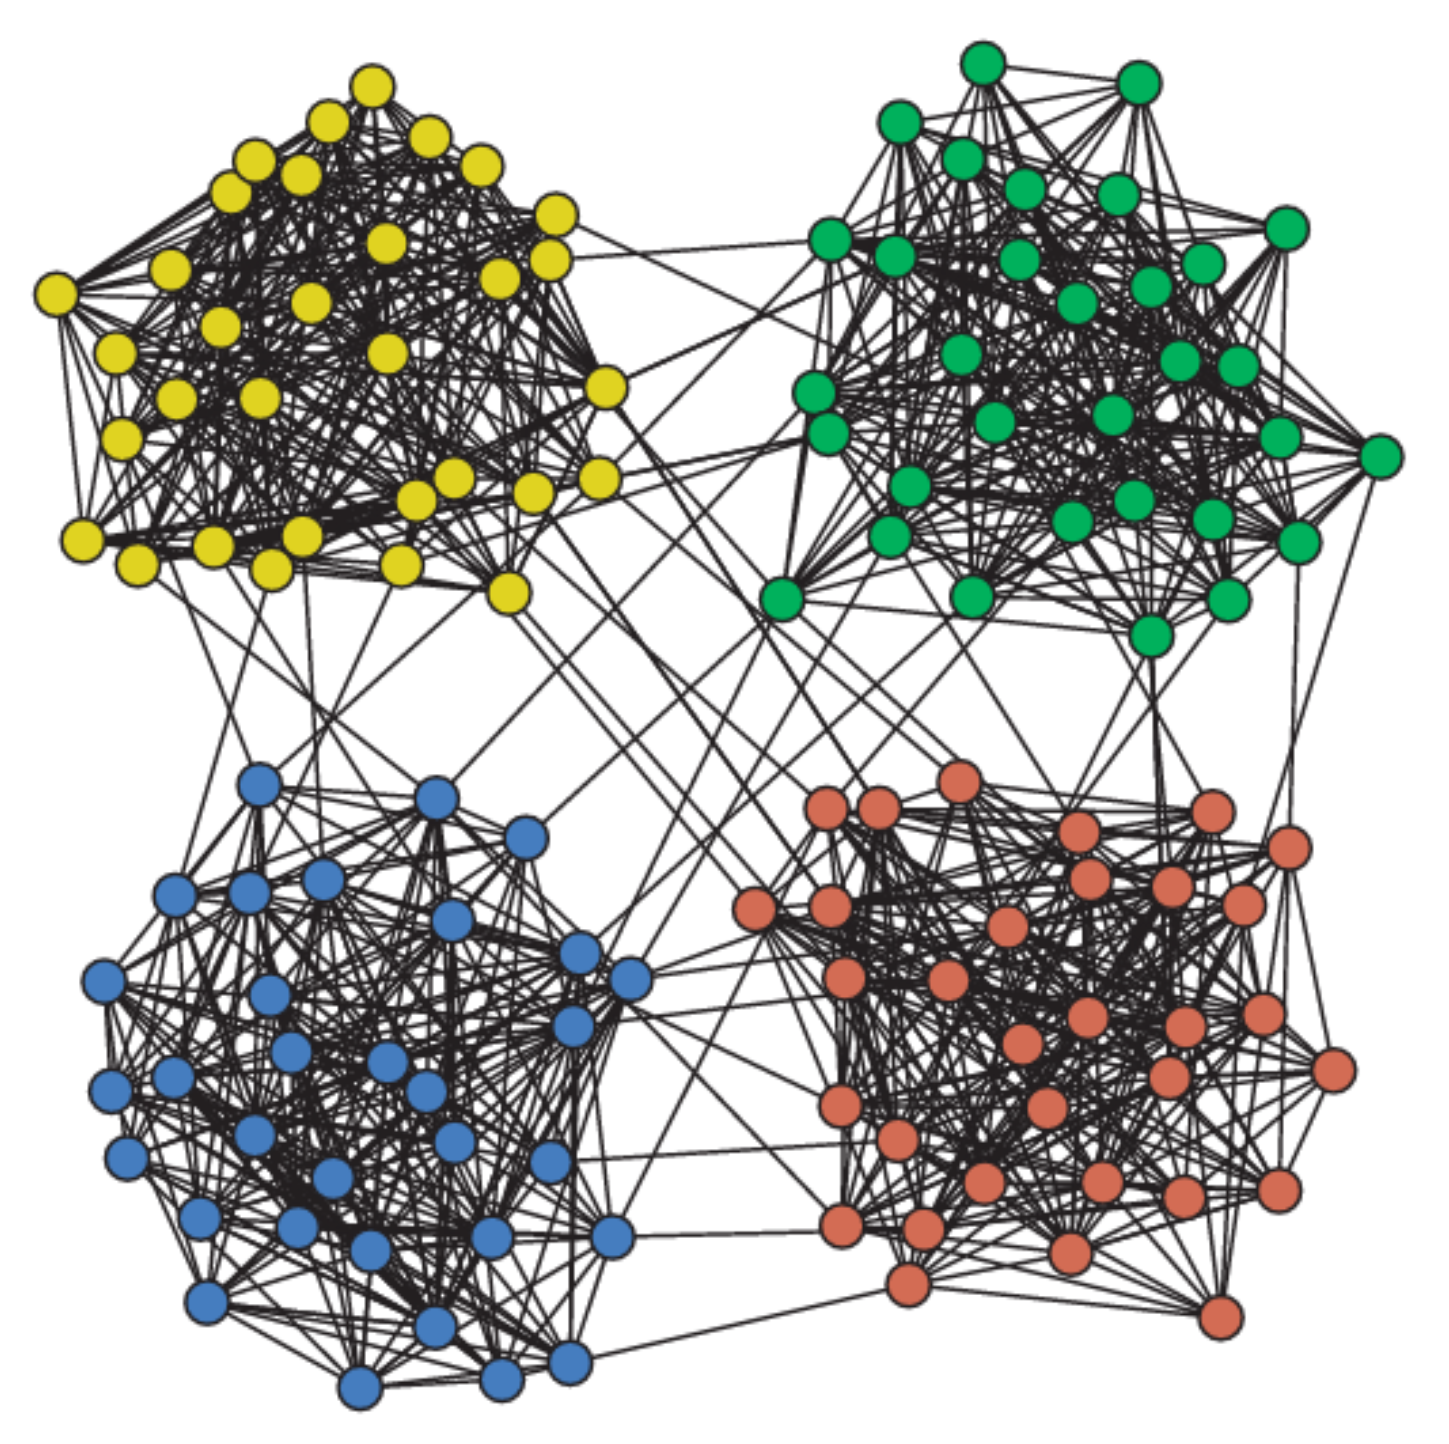
\includegraphics[width=1\linewidth]{figures/communities}
		\caption{\tiny Guimera, R., \& Amaral, L. (2005). Functional cartography of complex metabolic networks. Nature, 433, p. 896}
		\end{figure}
	\end{column}
\end{columns}

\end{frame}

%------------------------------------------------

\begin{frame}
\frametitle{User Activity: Retweet, Mentions and Replies}
\begin{figure}
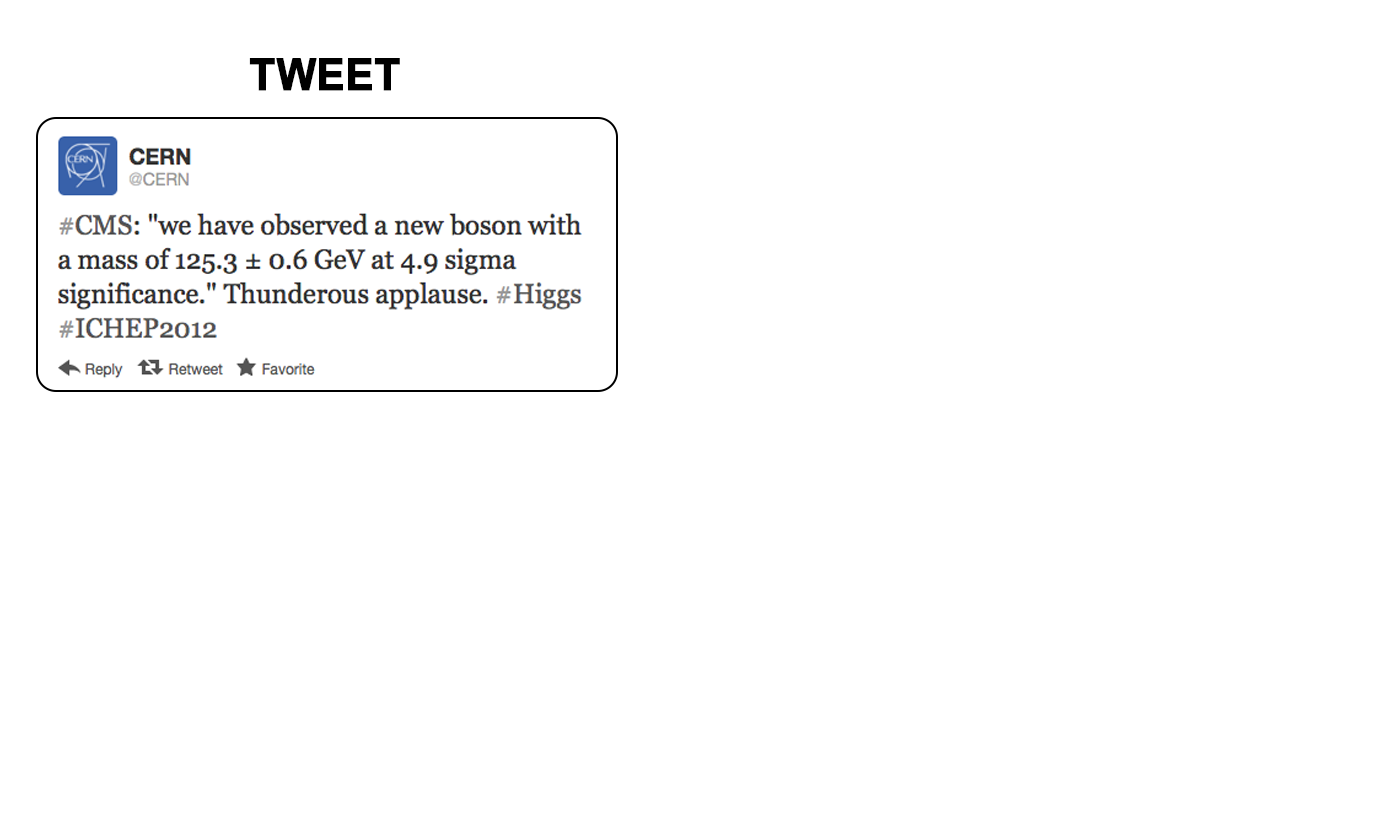
\includegraphics[width=1\linewidth]{figures/tweets/tweet}
\end{figure}
\end{frame}

\begin{frame}
\frametitle{User Activity: Retweet, Mentions and Replies}
\begin{figure}
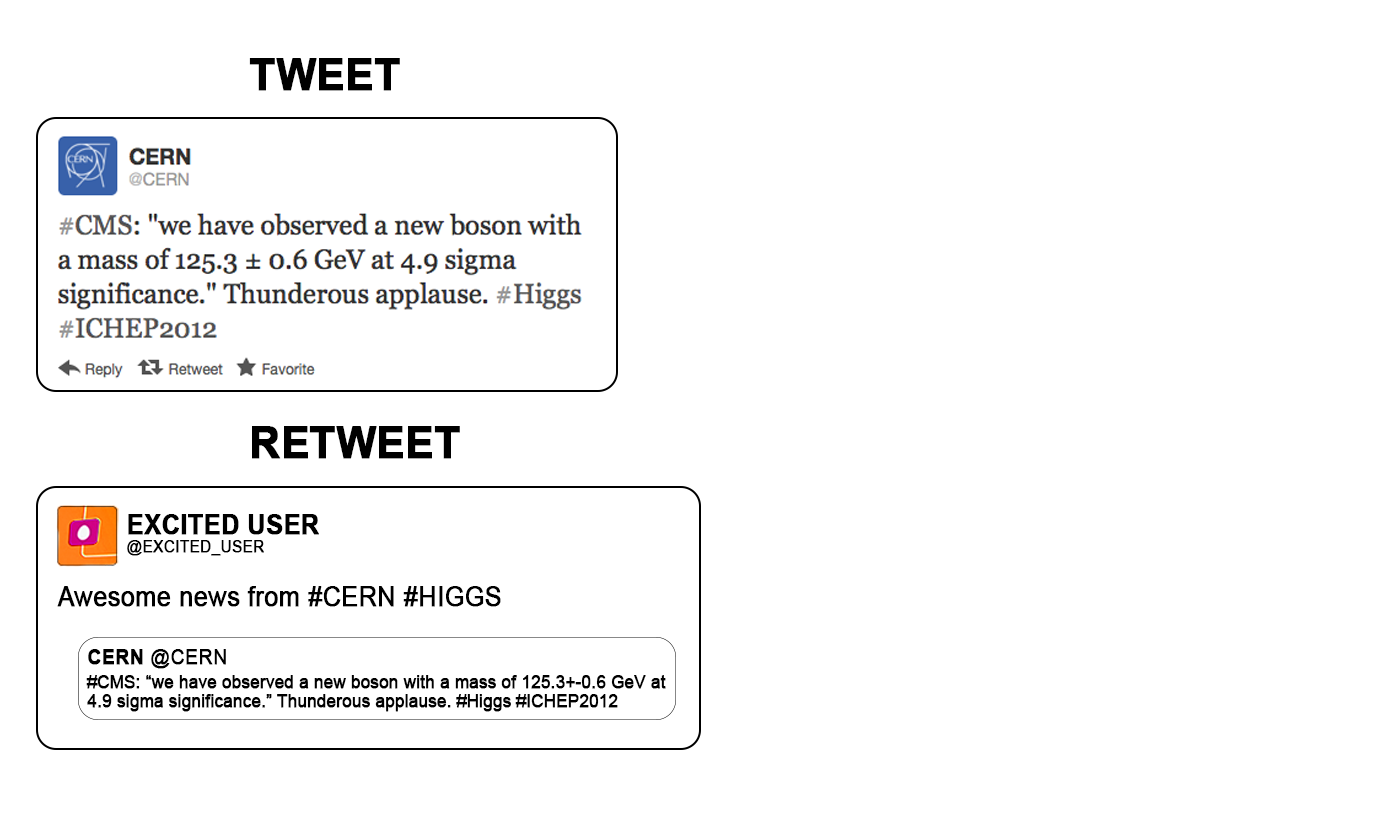
\includegraphics[width=1\linewidth]{figures/tweets/retweet}
\end{figure}
\end{frame}

\begin{frame}
\frametitle{User Activity: Retweet, Mentions and Replies}
\begin{figure}
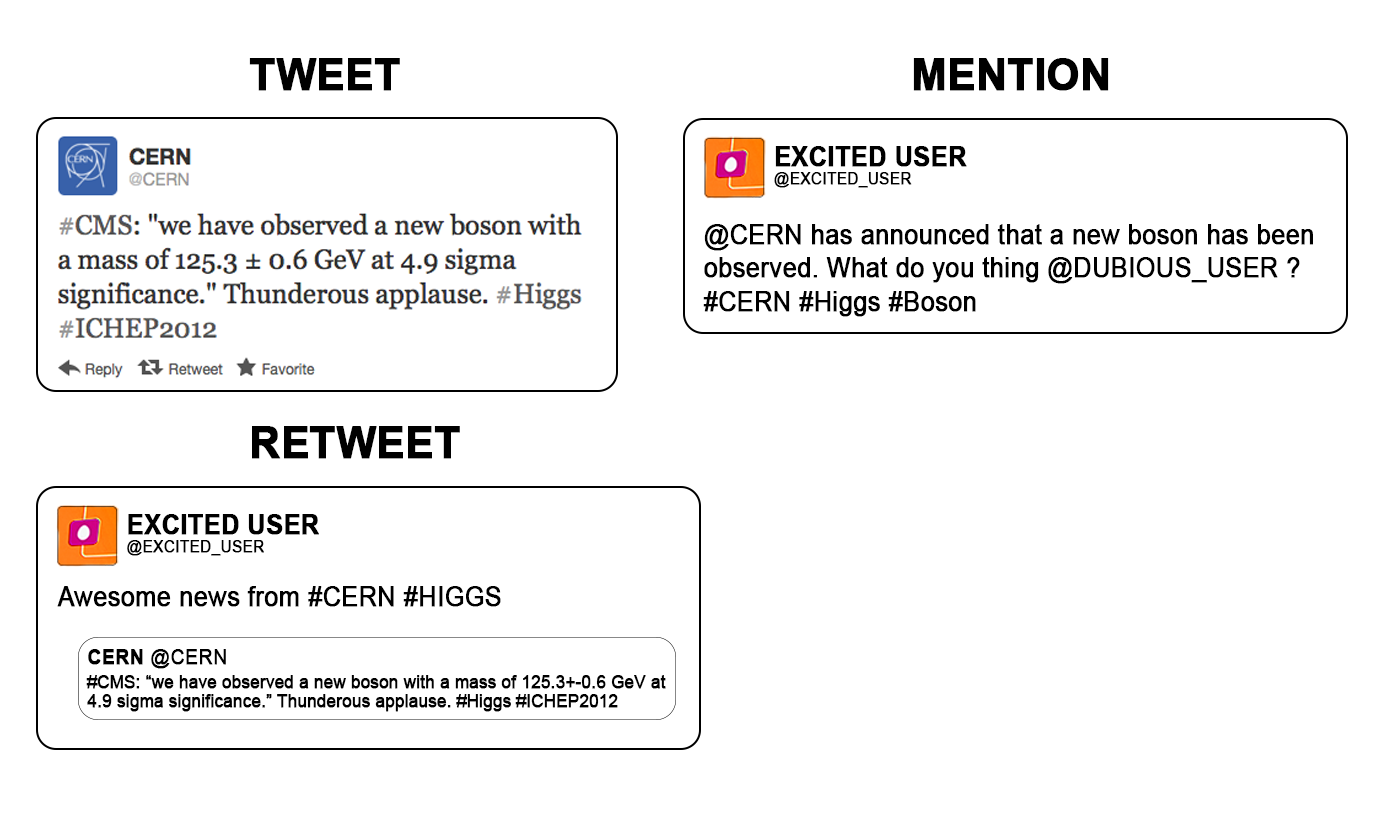
\includegraphics[width=1\linewidth]{figures/tweets/mention}
\end{figure}
\end{frame}

\begin{frame}
\frametitle{User Activity: Retweet, Mentions and Replies}
\begin{figure}
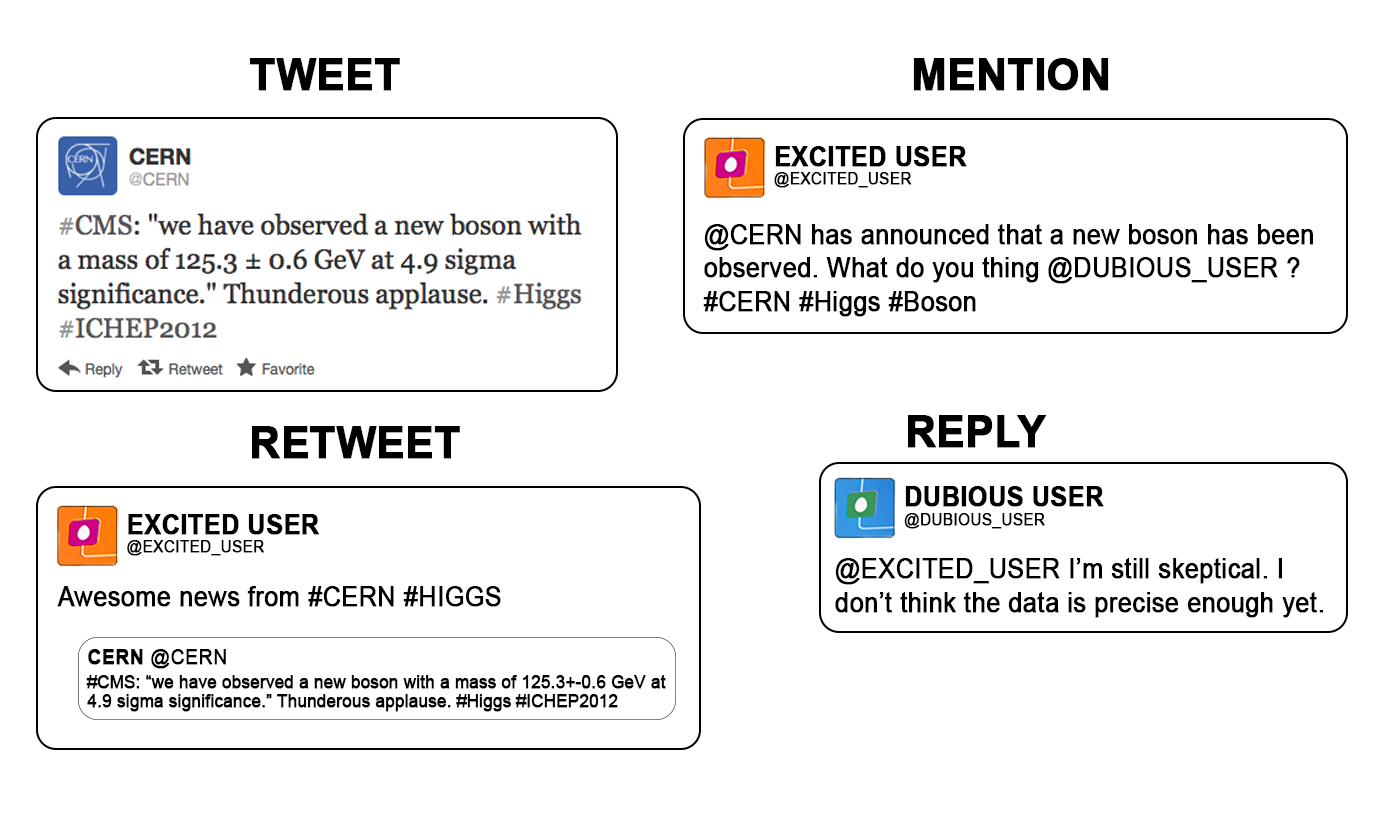
\includegraphics[width=1\linewidth]{figures/tweets/reply}
\end{figure}
\end{frame}

%------------------------------------------------

\begin{frame}
\frametitle{Community Activity}
\begin{columns}
	\begin{column}{0.3\textwidth}
	Community activity is divided into:
		\begin{itemize}
			\item Within (active) 
			\item Outgoing (active)
			\item Incoming (passive)
		\end{itemize}
	\end{column}
	\begin{column}{0.65\textwidth}
		\begin{figure}[r]
			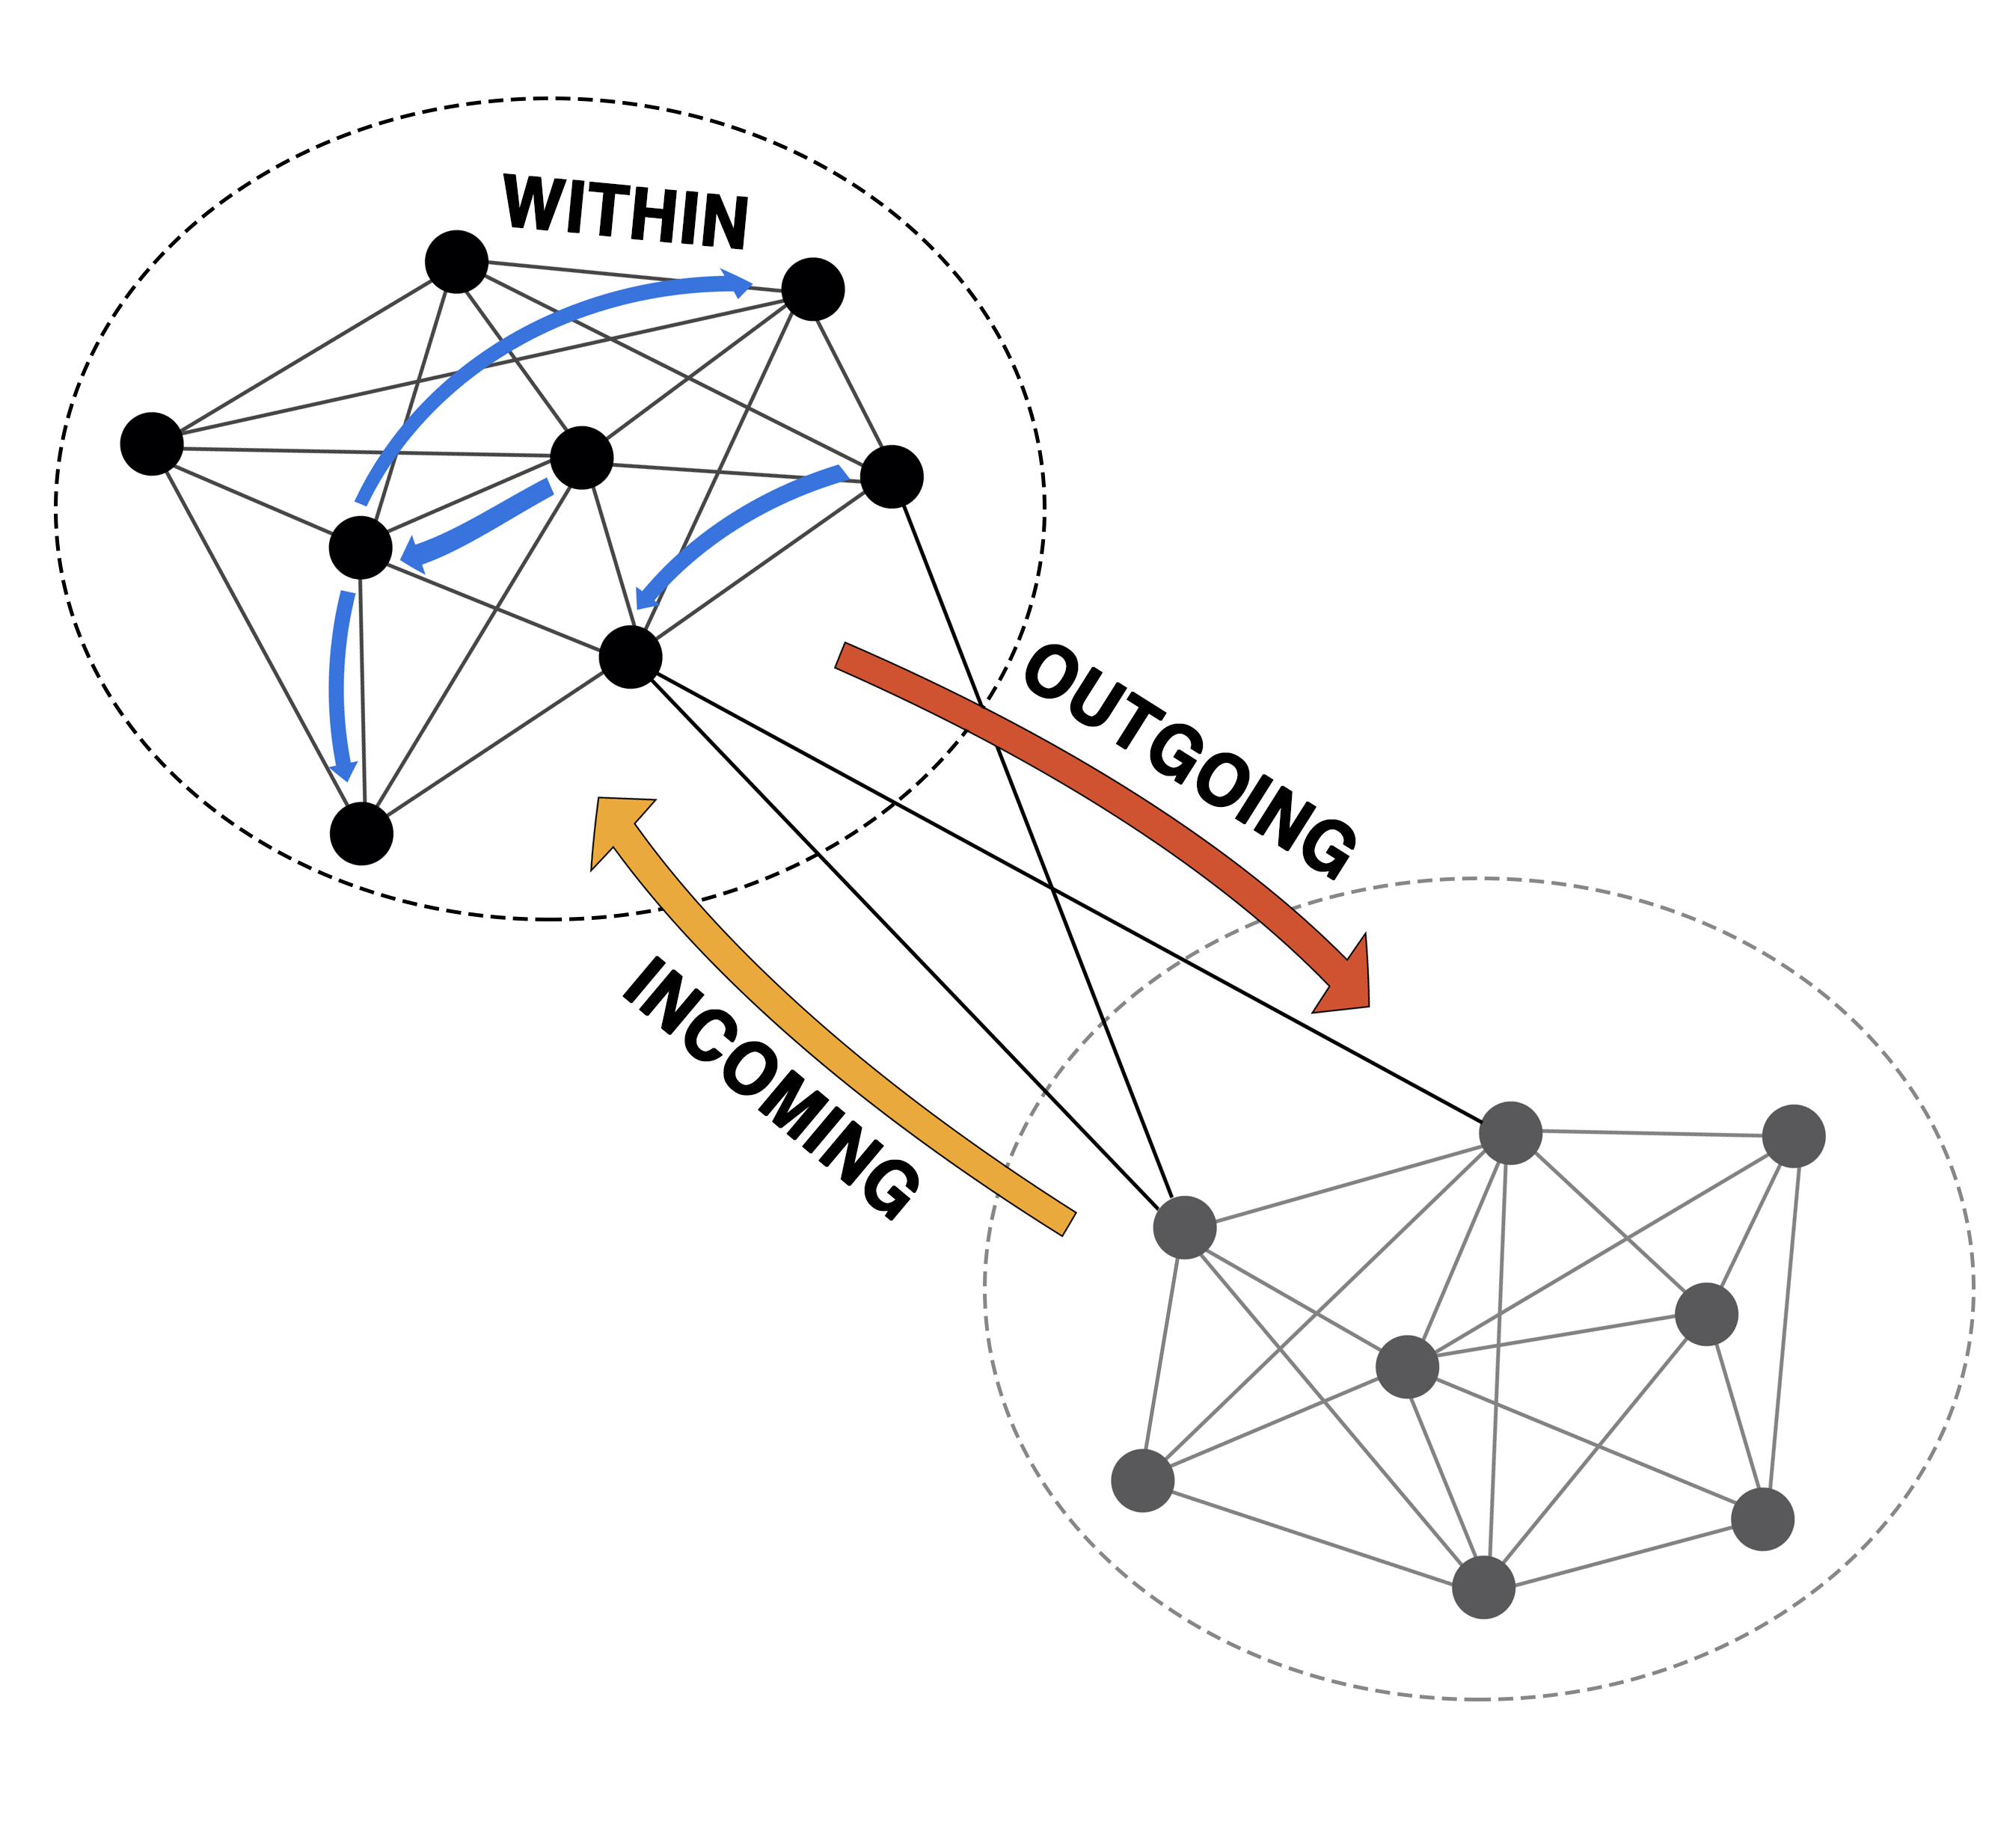
\includegraphics[width=1\linewidth]{figures/activity}
		\end{figure}
	\end{column}
\end{columns}
\end{frame}

%------------------------------------------------

\begin{frame}
\frametitle{Activity Classification: Index of Activity}
\begin{columns}
	\begin{column}{0.4\textwidth}
		\begin{figure}
			\vspace{-0.5cm}
			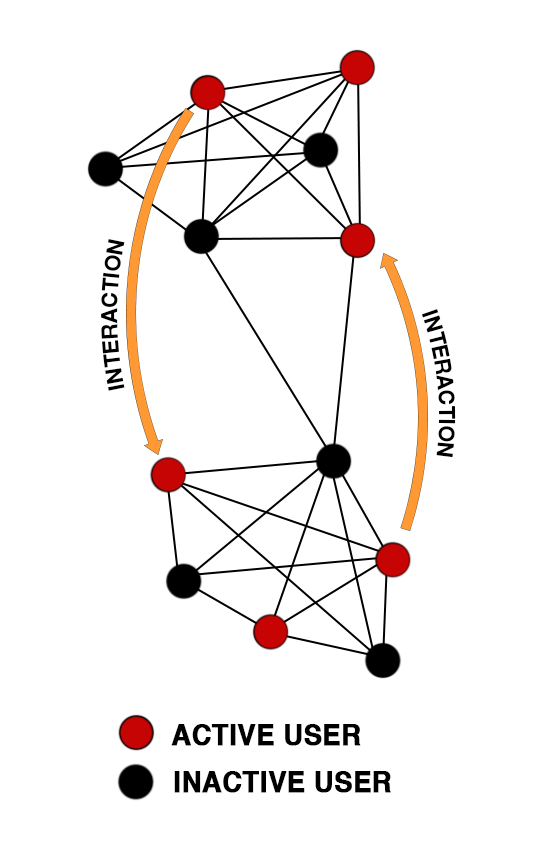
\includegraphics[width=1\linewidth]{figures/activeuser}
		\end{figure}
	\end{column}

	\begin{column}{0.6\textwidth}
		For each community we compute:
		\vspace{0.3cm}
		\begin{itemize}
			\item Number of Interactions 
			\item Number of Active Users
		\end{itemize}
		\vspace{0.3cm}
		and define the \textbf{Index of Activity} as
		\begin{figure}
			\centering
			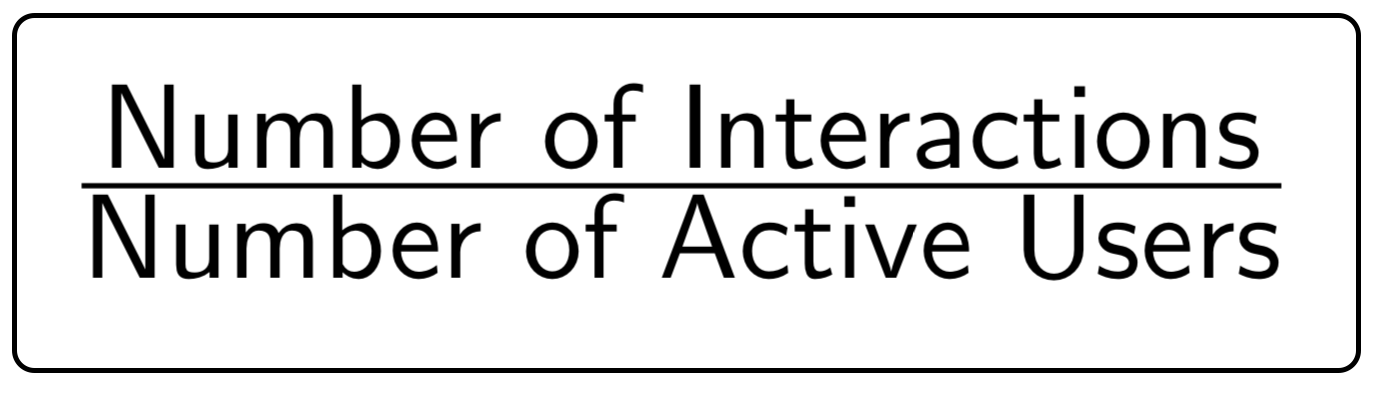
\includegraphics[width=0.85\linewidth]{figures/index}
		\end{figure}

	\end{column}
	
\end{columns}
\end{frame}

%------------------------------------------------

\begin{frame}
\frametitle{Community Detection Algorithm}
Choosing the right \textbf{community detection algorithm} is a crucial step of the network analysis. 
\vspace{0.5cm}

{
\centering 
\begin{tcolorbox}[width=8cm, colframe=black, colback=white, halign=center]
\textbf{CONSTANT POTTS MODEL} \small [1]
\end{tcolorbox}
}
\begin{itemize}
	\centering
	\item Able to unveil small sub-communities
	\centering
	\item Resolution parameter for smallest community size
\end{itemize}

\blfootnote{\small [1] Traag, V. A., Dooren, P. Van, Nesterov, Y. (2011). Narrow scope for resolution-limit-free community detection.}
\end{frame}

%------------------------------------------------

\begin{frame}
\frametitle{Computational Aspects: Tools}
\begin{itemize}
	\item \textbf{Community Detection}
	\begin{columns} 
		\begin{column}{0.5\textwidth}
		\begin{figure}
		
\includegraphics[width=0.6\linewidth]{figures/python1}
		\end{figure}
		\end{column}
		\begin{column}{0.5\textwidth}
		\begin{figure}
		
\includegraphics[width=0.6\linewidth]{figures/igraph}
		\end{figure}
		\end{column}
	\end{columns}
	\item \textbf{Community Analysis}
		\begin{columns} 
			\begin{column}{0.3\textwidth}
				\begin{figure}
				
\includegraphics[width=0.3\linewidth]{figures/cpiupiu}
				\end{figure}
			\end{column}
			\begin{column}{0.3\textwidth}
				\begin{figure}
				
\includegraphics[width=0.6\linewidth]{figures/awk}
				\end{figure}
			\end{column}
			\begin{column}{0.3\textwidth}
				\begin{figure}
				
\includegraphics[width=0.6\linewidth]{figures/bash}
				\end{figure}
			\end{column}
		\end{columns}
	\item \textbf{Plots and fits}
		\begin{columns}
			\begin{column}{0.5\textwidth}
				\begin{figure}
					
\includegraphics[width=0.7\linewidth]{figures/root}
				\end{figure}
			\end{column}
		\end{columns}
	\end{itemize}
\end{frame}

%------------------------------------------------

\begin{frame}
\frametitle{Total Activity (Active and Passive) \\ \normalsize $\blacksquare$ Activity is constant for small communities }
\begin{figure}
	\vspace*{-0.1cm}
	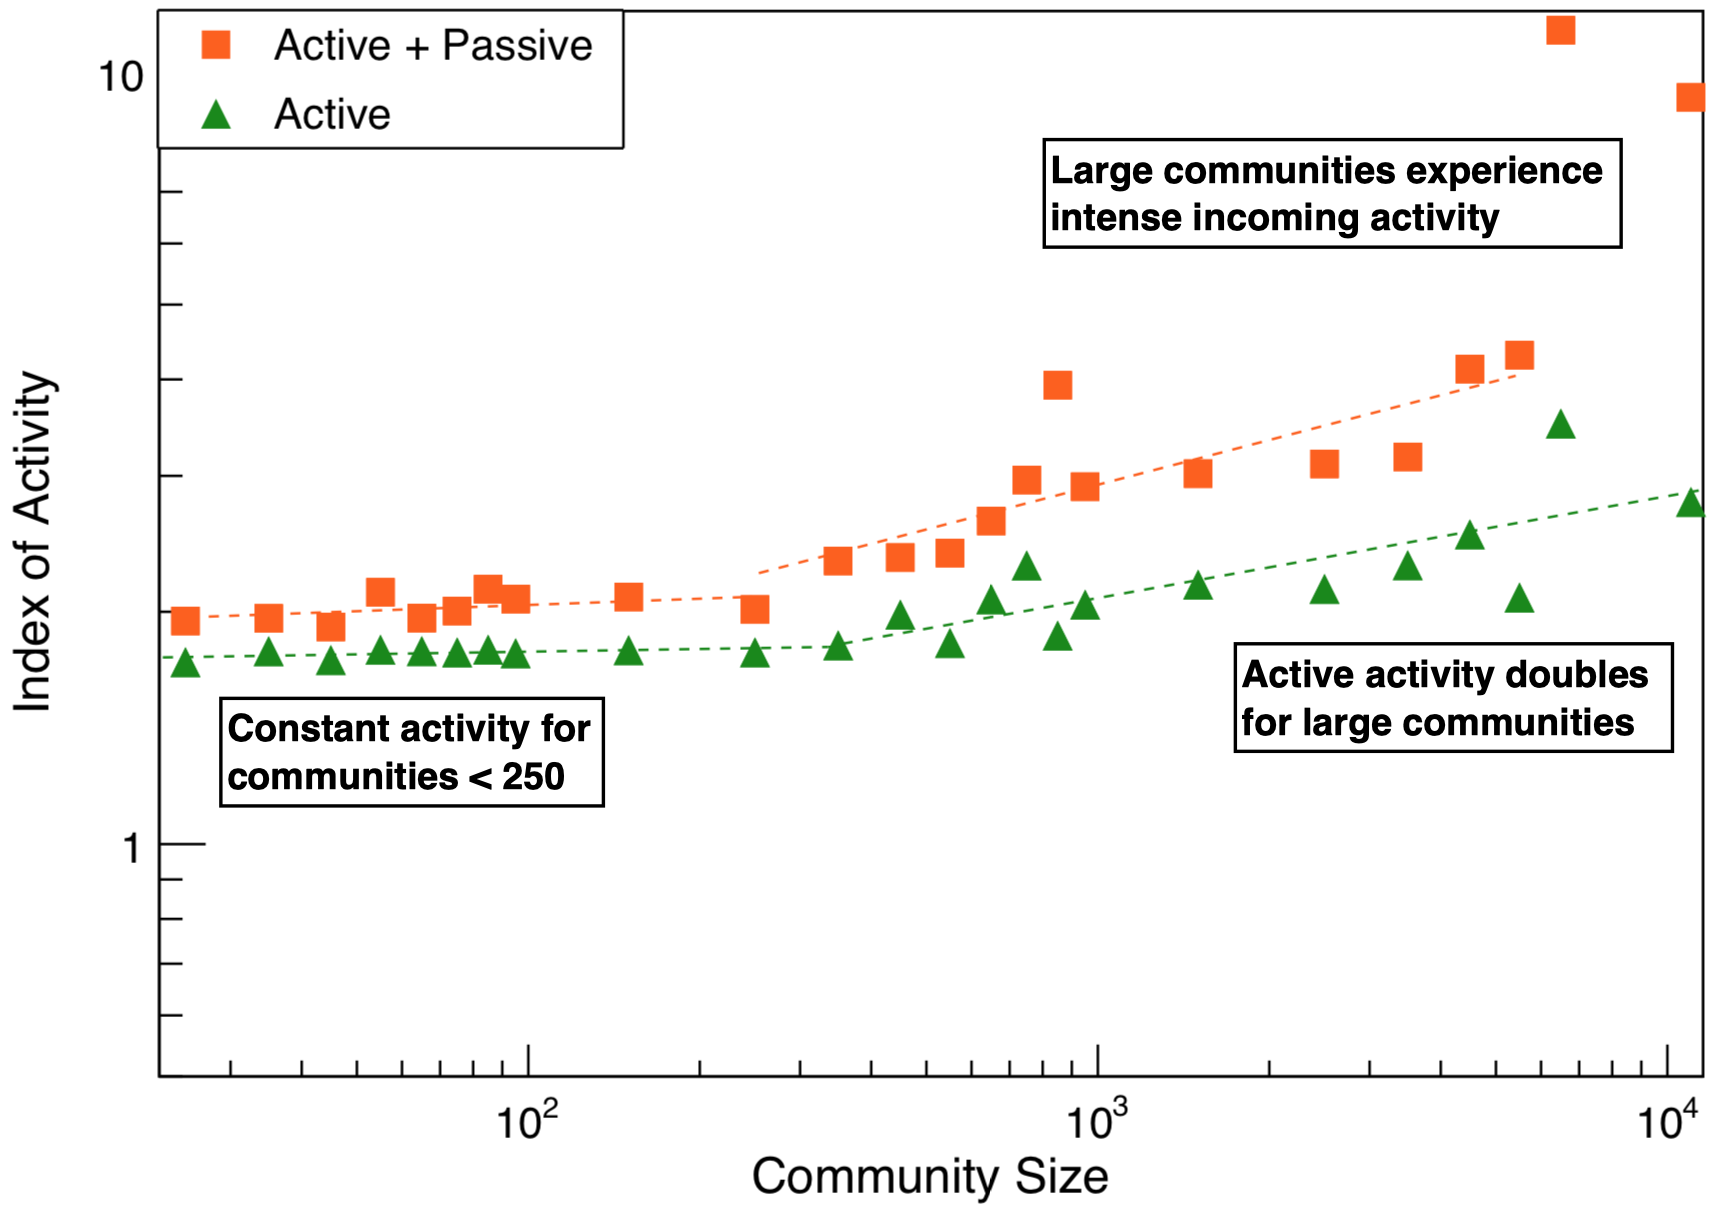
\includegraphics[width=0.8\linewidth]{figures/activity/total}
\end{figure}
\small Trend lines are for guidance only

\end{frame}

%------------------------------------------------

\begin{frame}
\frametitle{Total Activity by Community Interaction \\ \normalsize $\blacksquare$ Outgoing activity decreases with cluster size}

\begin{figure}
	\vspace*{-0.1cm}
	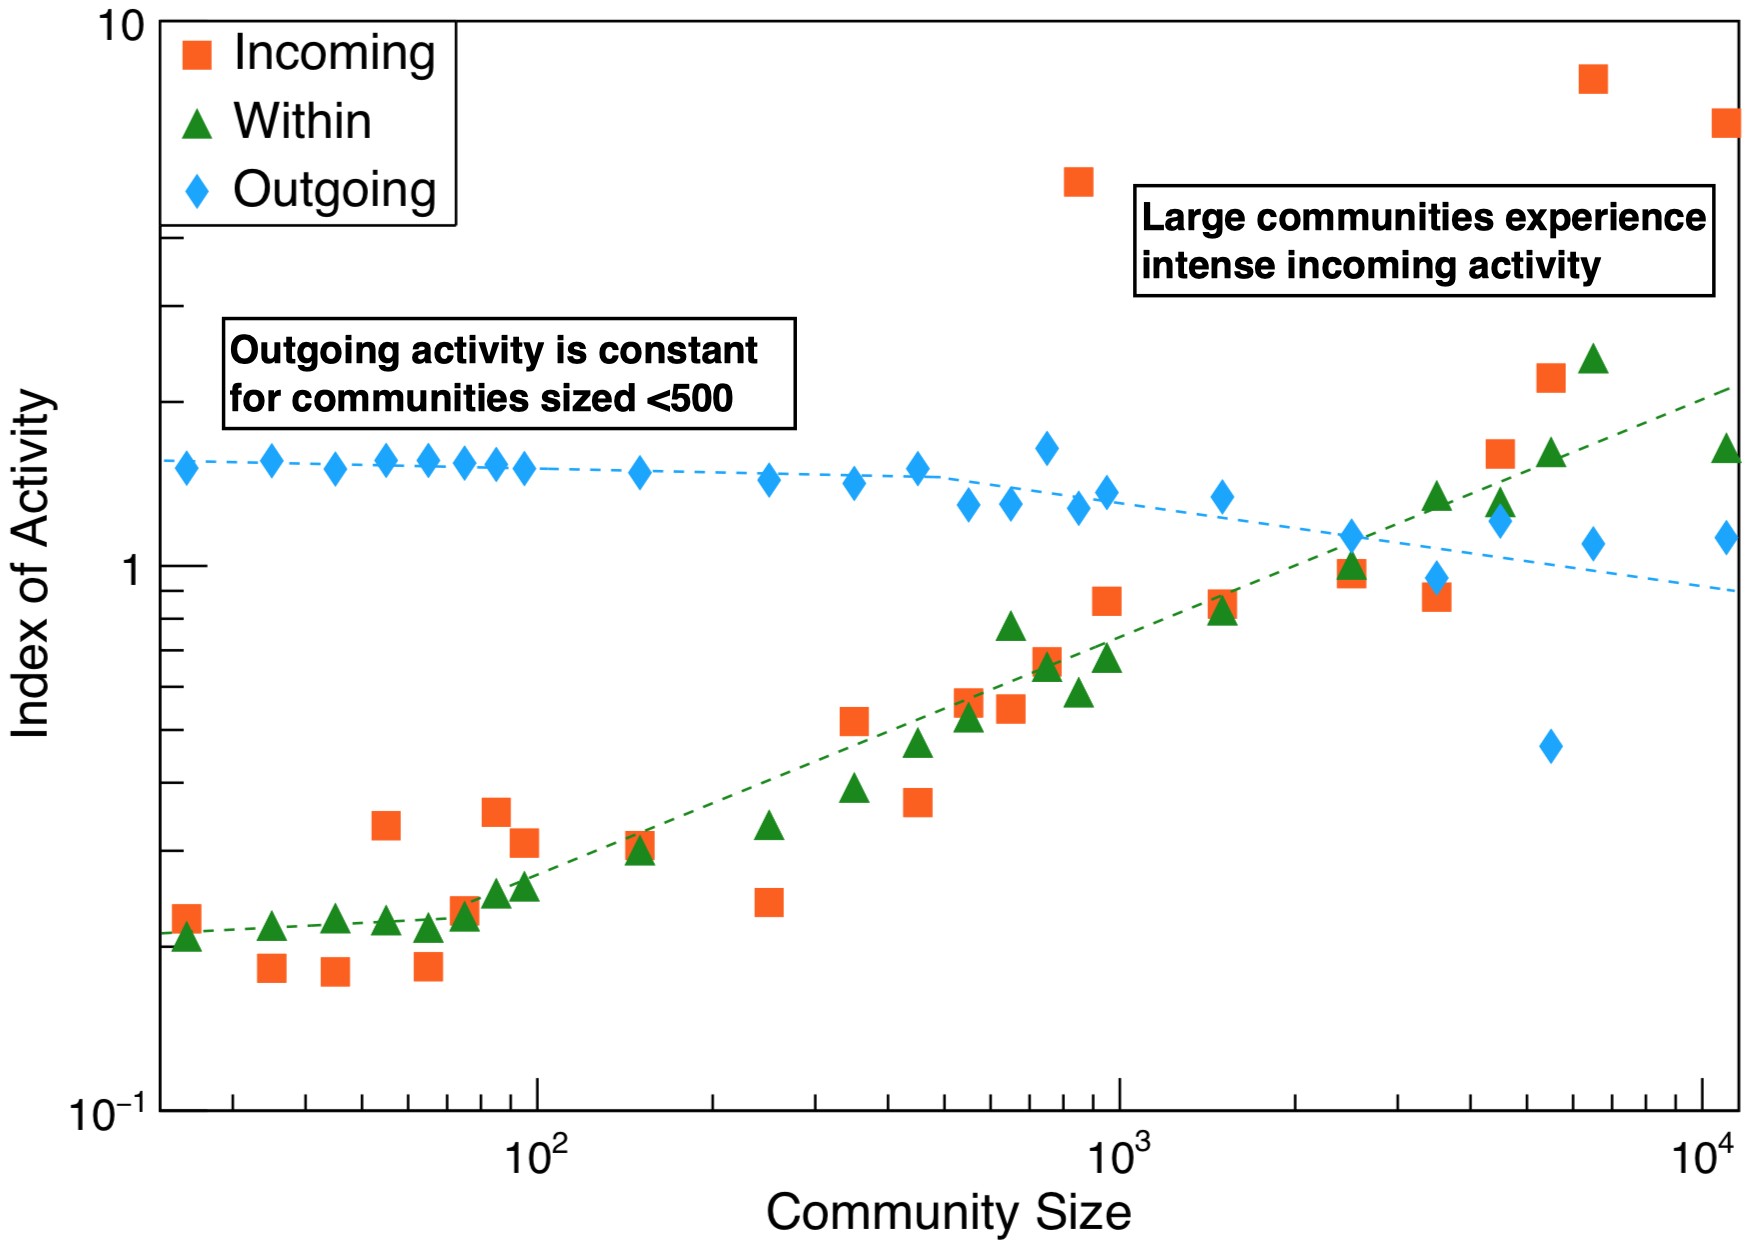
\includegraphics[width=0.79\linewidth]{figures/activity/total_by_type}
\end{figure}
\small Trend lines are for guidance only

\end{frame}

%-----------------------------------------------

\begin{frame}
\frametitle{Outgoing Activity by Type of User Interaction \\ \normalsize $\blacksquare$ Mention activity is constant}
\begin{figure}
	\vspace*{-0.1cm}
	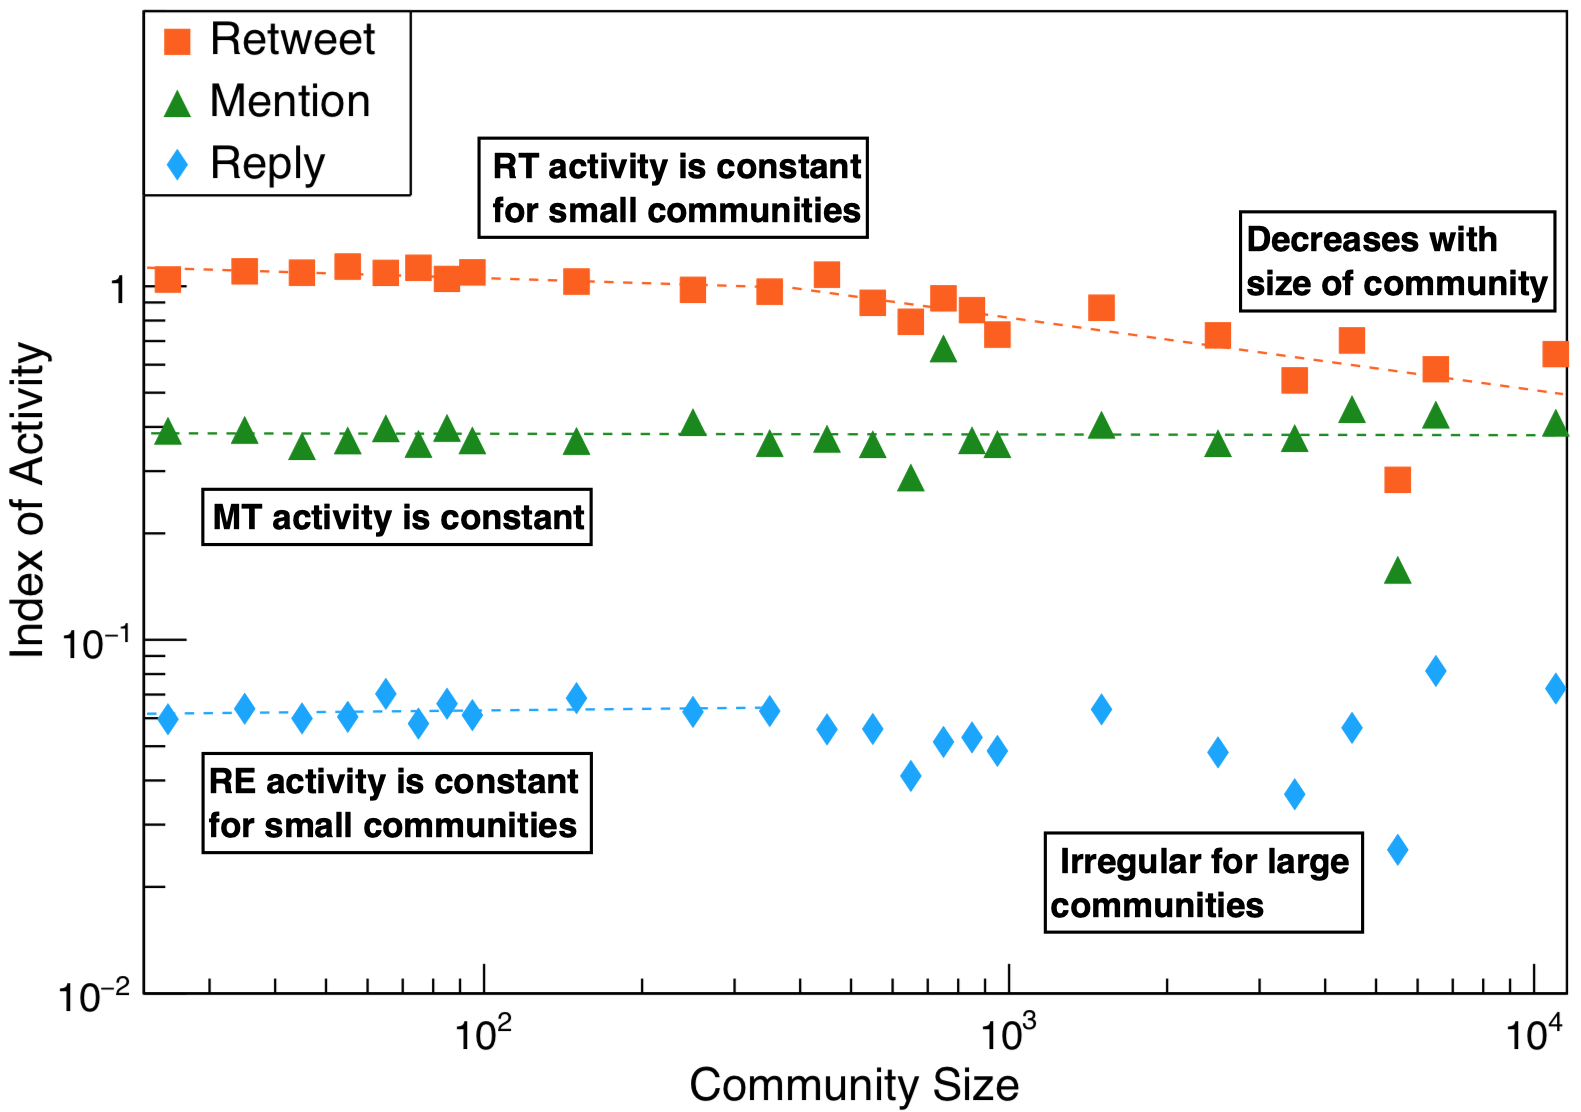
\includegraphics[width=0.8\linewidth]{figures/activity/outgoing}
\end{figure}
\small Trend lines are for guidance only

\end{frame}

%-----------------------------------------------

\begin{frame}
\frametitle{Within Activity by Type of User Interaction \\ \normalsize $\blacksquare$ Retweet and Mention activity increase at the same rate}
\begin{figure}[t]
	\vspace*{-0.1cm}
	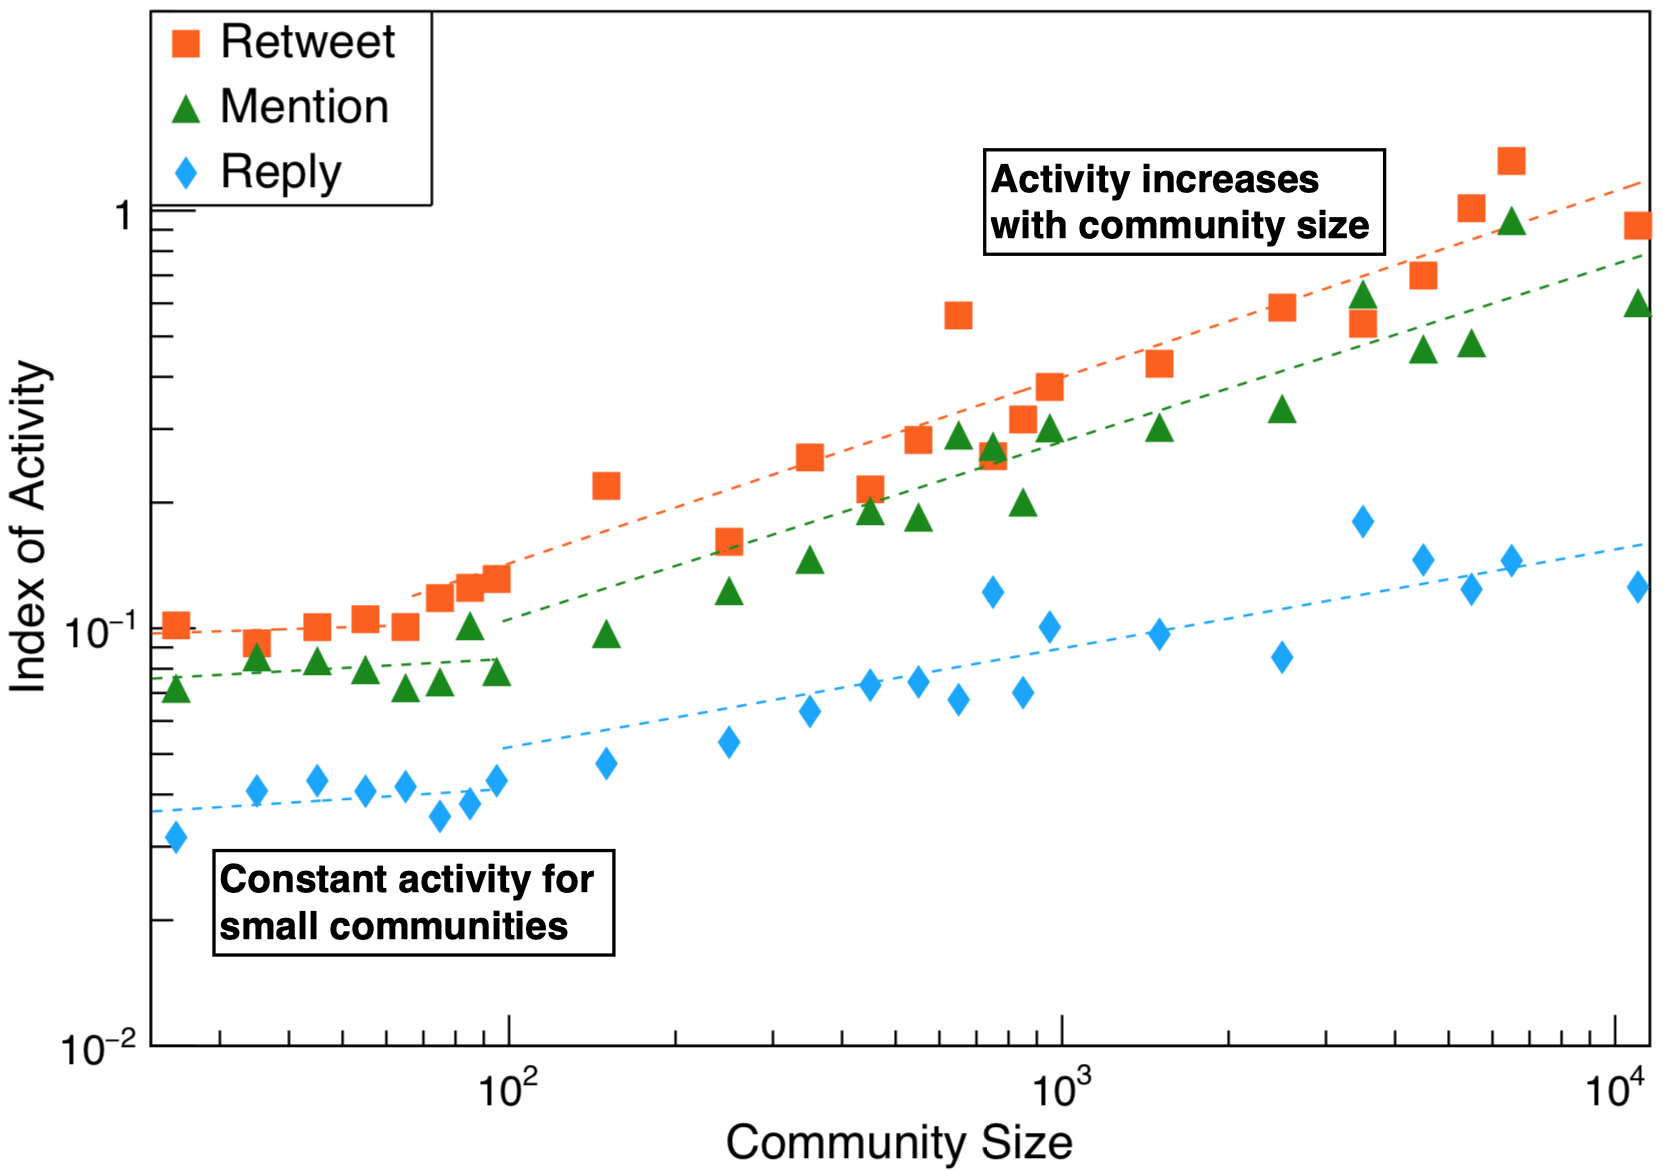
\includegraphics[width=0.8\linewidth]{figures/activity/within}
\end{figure}
\small Trend lines are for guidance only
 
\end{frame}

%-----------------------------------------------

\begin{frame}
\frametitle{Incoming Activity by Type of User Interaction \\ \normalsize $\blacksquare$ Activity increases with community size}
\begin{figure}
	\vspace*{-0.1cm}
	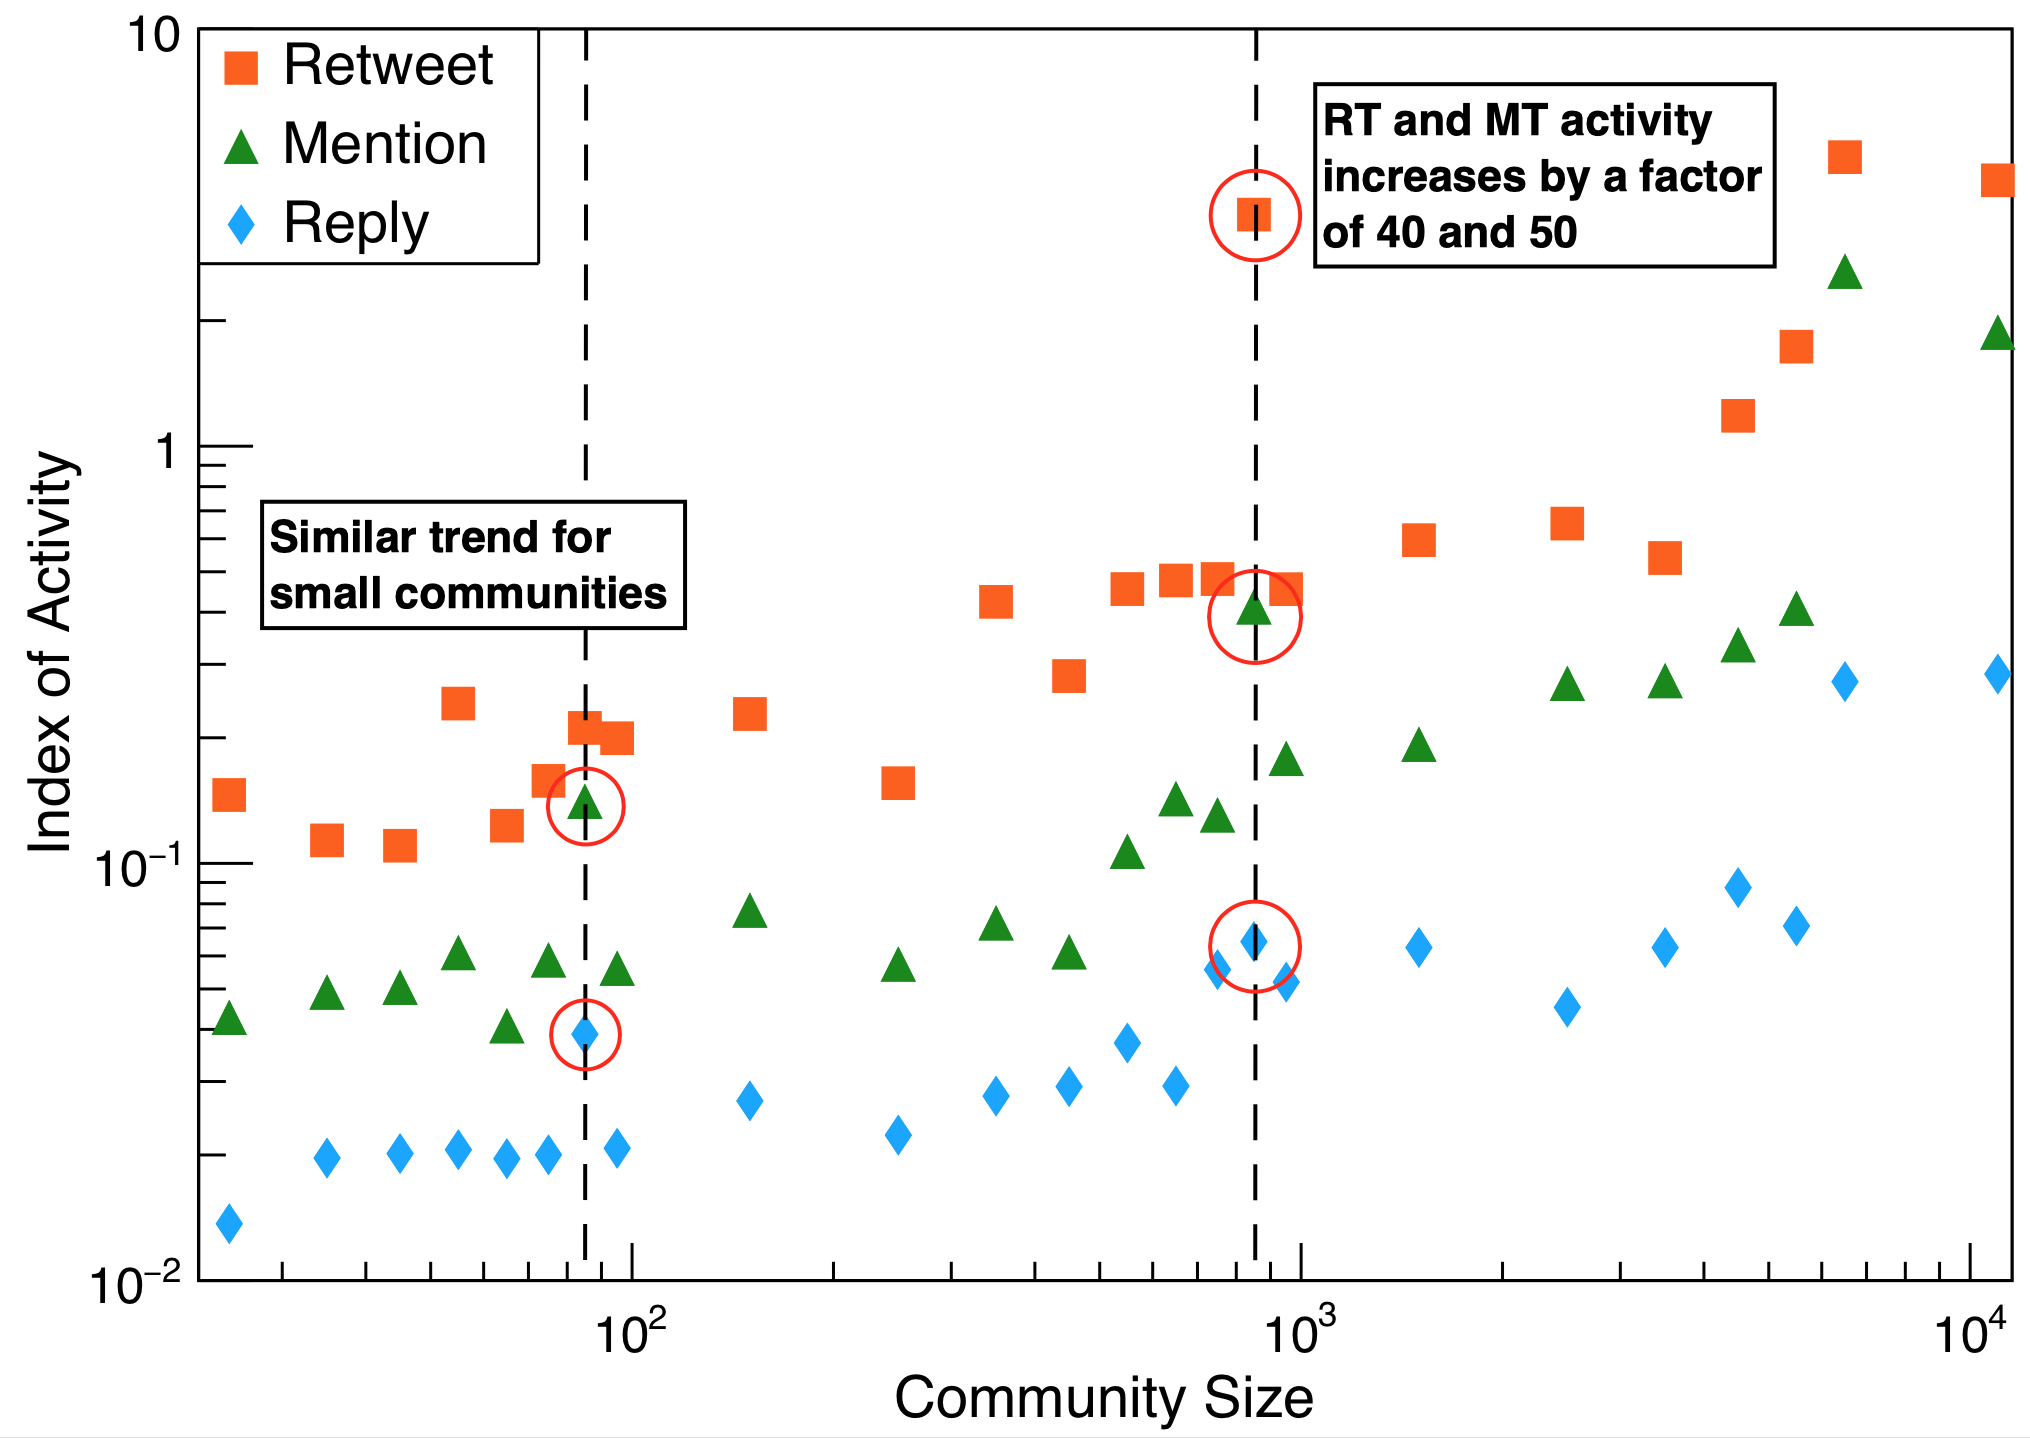
\includegraphics[width=0.8\linewidth]{figures/activity/incoming}
\end{figure}
\end{frame}

%-----------------------------------------------

\begin{frame}
\frametitle{What do these results tell us?}
	\begin{enumerate}
		\item \large \textbf{Small} communities (less than 150-350 users) show similar activity, regardless of the type
		\vspace{0.5cm}
		\item \large For \textbf{large} communities the activity increases/decreases with the community size 
		\begin{itemize}
			\item Increases for Within and Incoming Activity
			\item Decreases for Outgoing Activity
			\vspace{0.5cm}
			\item \textbf{Exception}: \underline{Outgoing Mentions Activity} is constant for all communities
		\end{itemize}
	\end{enumerate}
\end{frame}

%-----------------------------------------------

\begin{frame}
\frametitle{What do these results tell us?}

\begin{columns}
	\begin{column}[T]{0.4\textwidth}
	{
	\centering
	\begin{tcolorbox}[width=3cm, colframe=black, colback=white, halign=center]
	\textbf{SMALL} 
	\end{tcolorbox}
	}

	\begin{itemize}
		\item \textbf{Less} activity \textbf{within} the community
		\vspace{0.4cm}
		\item Very \textbf{little} \textbf{incoming} activity
		\vspace{0.4cm}
		\item \textbf{More} activity is directed outside the community (\textbf{outgoing})
		
	\end{itemize}
	\end{column}


	\begin{column}[T]{0.4\textwidth}
	{
	\centering
	\begin{tcolorbox}[width=3cm, colframe=black, colback=white, halign=center]
	\textbf{LARGE}
	\end{tcolorbox}
	}
	\begin{itemize}
		\item \textbf{More} activity \textbf{within} the community 
		\vspace{0.4cm}
		\item \textbf{Less} \textbf{outgoing} activity
		\vspace{0.4cm}
		\item Experience \textbf{intense} \textbf{incoming} activity
	\end{itemize}
	\end{column}
\end{columns}
\end{frame}
%-----------------------------------------------

\begin{frame}
\frametitle{Lessons Learned}

\begin{itemize}
	\item \textbf{Retweets} are the \textbf{most frequent} type of interaction, suggesting that the \textbf{news} is \textbf{shared} rather than discussed
	\vspace{0.5cm}
	\item \textbf{Small communities} activity is \textbf{directed towards} other communities, probably of larger size 
	\vspace{0.5cm}
	\item During an \textbf{extraordinary event} the activity is \textbf{not contained} within the community, but spreads through the network 
\end{itemize}
\end{frame}

%-----------------------------------------------

\begin{frame}
\frametitle{Future Developments}

\begin{itemize}
	\Large
	\item \large\textbf{SPATIAL ANALYSIS}
	\vspace{0.2cm}
	\begin{itemize}
	\item \large Where is the outgoing activity directed to?
	\end{itemize}
	\vspace{0.5cm}

	\item \large\textbf{TEMPORAL ANALYSIS}
	\vspace{0.2cm}
	\begin{itemize}
		\item Burst of activity
		\item Time of activation
	\end{itemize}
\end{itemize}
\end{frame}

%------------------------------------------------

\begin{frame}

\begin{columns}
	\begin{column}{0.47\textwidth}
	\centering
		\textbf{Thanks for your attention}
	\end{column}
	\begin{column}{0.5\textwidth}
		\begin{figure}
		\centering
			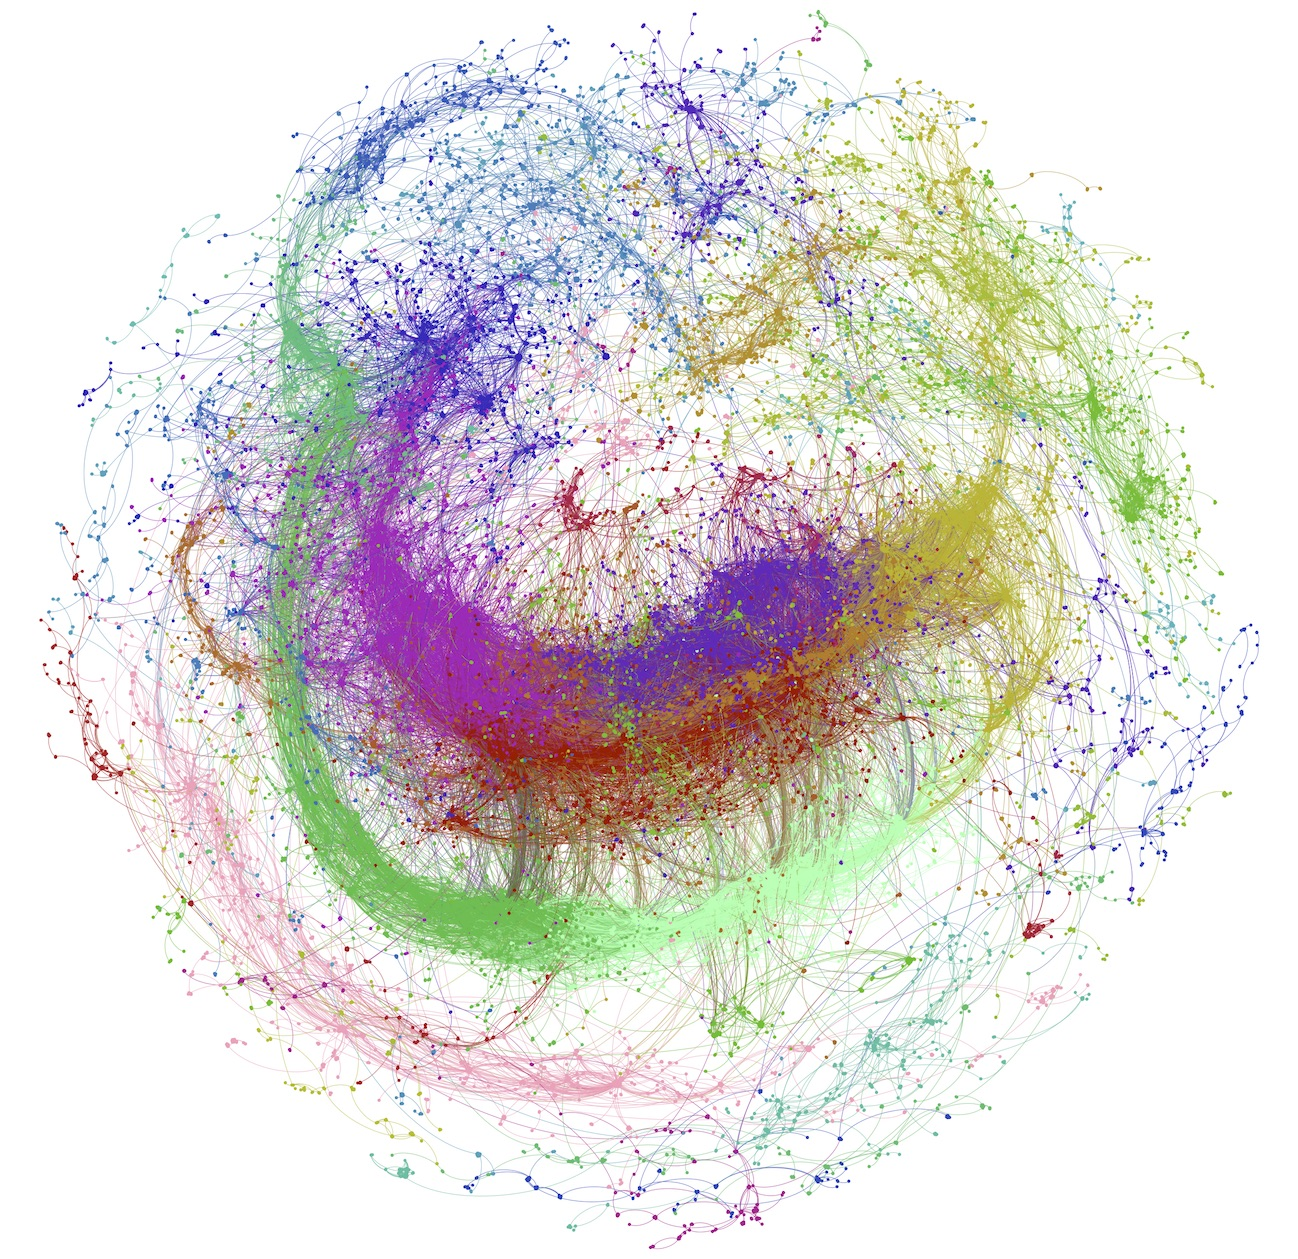
\includegraphics[width=1\linewidth]{fig7}
		\caption{\tiny Benzi, K., Ricaud, B., Vandergheynst, P., et Traitement, L. De. (2016). Principal Patterns on Graphs : Discovering Coherent Structures in Datasets, 1–19.}
		\end{figure}
	\end{column}
\end{columns}

\end{frame}
%----------------------------------------------------------------------------------------













\end{document} 